% Todo:

\documentclass[12pt]{article}
\usepackage[no-math]{fontspec}	% no-math option required for accents package
\usepackage{hyperref}
\usepackage{xeCJK}
%\setCJKmainfont{SimSun}
\setCJKmainfont[BoldFont=SimHei,ItalicFont=KaiTi]{SimSun}
% \setCJKsansfont{SimHei}
% \setCJKmonofont{SimKai}
\setmainfont{Arial}

\usepackage{accents}		% for dots under Chinese for empahsis
\usepackage{cite}
\usepackage{graphicx}
\usepackage{float}
\usepackage{amsfonts}
% \usepackage{amsmath}	% for \tag
\usepackage{amssymb}	% for \multimap
% \usepackage{stmaryrd}
\usepackage{color}
%\usepackage[square,numbers]{natbib}
%\nocopyright
%\usepackage{latexsym,amsmath,amssymb,graphicx,hyperref}
%\usepackage{times} % gives you a bit more space if needed
\usepackage{titlesec}		% change color of section headings
\usepackage{verbatim}		% enables to define {comment} blocks
%\usepackage[most]{tcolorbox}		% color box

% Left and right angle brackets
\makeatletter
\newsavebox{\@brx}
\newcommand{\llangle}[1][]{\savebox{\@brx}{\(\m@th{#1\langle}\)}%
  \mathopen{\copy\@brx\kern-0.5\wd\@brx\usebox{\@brx}}}
\newcommand{\rrangle}[1][]{\savebox{\@brx}{\(\m@th{#1\rangle}\)}%
  \mathclose{\copy\@brx\kern-0.5\wd\@brx\usebox{\@brx}}}
\makeatother

% Make dots under Chinese characters for emphasis
\renewcommand{\d}[1]{$\underaccent{\scalebox{0.4}{\textbullet}}{\textrm{#1}}$}
\makeatletter\newcommand{\ds}[1]{\@tfor\next:=#1\do{\d{\next}}}\makeatother

\titleformat{\section}
{\color{blue}\normalfont\Large\bfseries}
{\color{blue}\thesection}{1em}{}
\titleformat{\subsection}
{\color{blue}\normalfont\large\bfseries}
{\color{blue}\thesubsection}{1em}{}

\renewcommand\abstractname{\textcolor{blue}{Abstract}}

\definecolor{LogicColor}{rgb}{0.4,0.1,0.4}  % Magenta
\definecolor{Hilight}{rgb}{0.9,0.9,0.8}  % Magenta
% \definecolor{LogicColor}{rgb}{0,0,0}	% for black-and-white paper

\newcommand{\concept}[1]{\textbf{\textcolor{blue}{#1}}}

\newcommand{\english}[1]{\rmfamily \textit{``#1''}\rmfamily}
\newcommand{\formula}[1]{\textcolor{LogicColor}{#1}}

\newcommand{\hilight}[1]{\begin{tcolorbox}[breakable]#1\end{tcolorbox}}

\newcommand{\tab}{\hspace*{1cm}}

\newcommand*\sigmoid{\vcenter{\hbox{
\includegraphics{sigmoid.png}}}}
\newcommand*\sadface{
\includegraphics[scale=0.25]{face-sad.png}}

\setlength{\oddsidemargin}{1cm}
\setlength{\evensidemargin}{1cm}
\setlength{\textwidth}{14cm}

\linespread{1.2}

\title{\textcolor{blue}{Genifer 5.0 理论笔记}}
\author{YKY (\textit{甄景贤})}
%% \date{30 June 2015}
%% \institute{}

\begin{document}

\begin{comment}
\tab\tab\tab \parbox{9cm}{\textit{.....}}
% \vspace{-0.5cm}
\begin{flushright}
\textemdash\, .... \hspace*{2cm}
\end{flushright}
\end{comment}

% \sffamily

{\let\newpage\relax\maketitle}

\maketitle
\setlength{\parindent}{0em}
\setlength{\parskip}{1.5ex plus0.5ex minus1.2ex}

\section{新 model}

和 Joseph Cheng 谈过之后,发觉进一步简化比较好:

\subsection{放弃 sentence structure}

因为太麻烦了,增加复杂性。  想像一个只能用单字说话的 baby,如果她将来够聪明的话,她可以学会用单字组成句子,但那要视乎她内部知识的增长。 这些语言方面的知识,我们不会 externally program 进去。 宁愿她开始时比较低能,也好过我们 design 到筋疲力尽。

回顾一下我们的 neural reasoner model:
\begin{figure}[H]
\centering
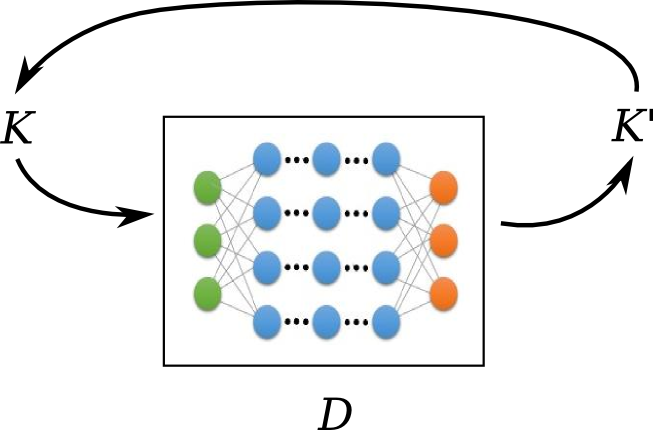
\includegraphics[scale=0.75]{genifer-model-0.png}
\end{figure}

新的 cognitive state vector $K$ 可以是这样的:
\begin{figure}[H]
\centering
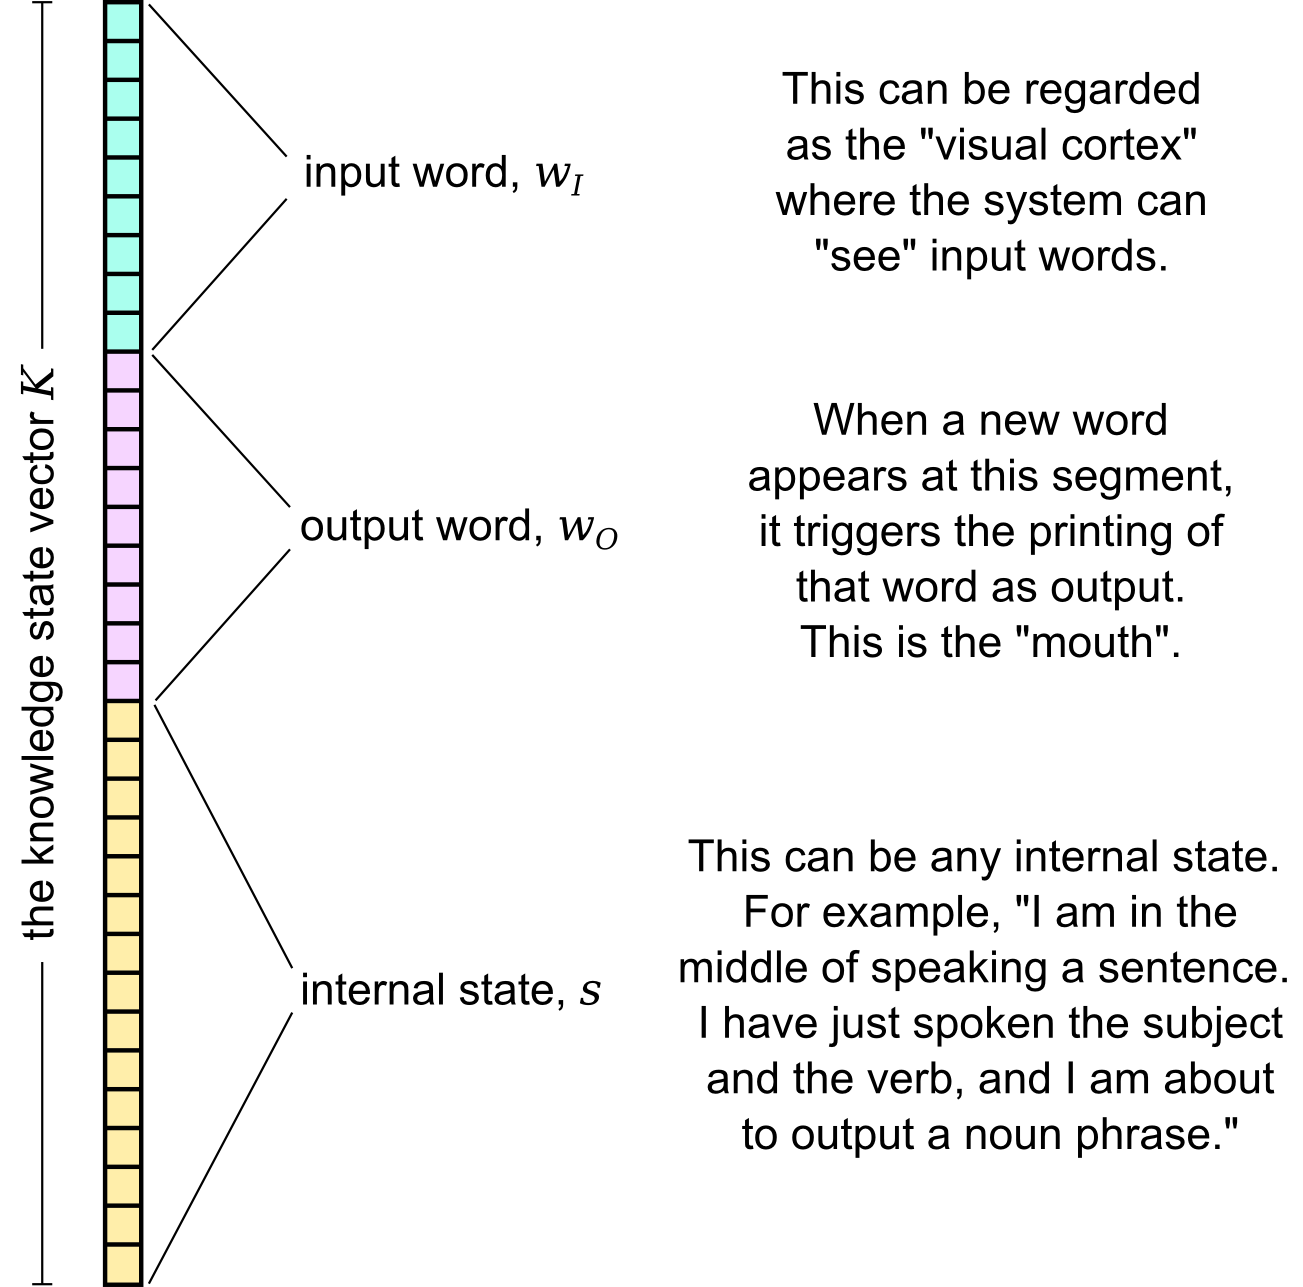
\includegraphics[scale=0.75]{internal-state-K.png}
\end{figure}

$w_I$ 和 $w_O$ 分别是 Genifer 的「眼」和「口」。

$w_I$ 可以是 word2vec 产生的 vector,这里我们只是利用 word2vec 输出的 representation,算法基本上是和 word2vec 无关的。

$w_O$ 是 reasoner 的输出,每当这部分变动时,我们就印出一个新的字。 

$s$ 是「内部状态」,也可以叫 \,"working memory" (认知科学术语),也可以看成是 Turing machine 里的记忆磁带。 它记住当前的问题状态,$D$ 作用在 $K$ 之上,产生新的结论。

\subsection{用 reinforcement learning 控制 logic reasoner}

好处是不需人手。 



$D$ 不变,$K_0$ 是已知的,求 $K_\infty$:
$$ K_0 \stackrel{D}{\longrightarrow} K_1 \stackrel{D}{\longrightarrow} .... \; K_\infty $$

\begin{eqnarray}
K_0 & \stackrel{D}{\longrightarrow} & .... \; K_\infty \nonumber \\
\mbox{error } \mathcal{E} & = & K_\infty - K^* \nonumber \\
\mbox{minimize error, with gradient} & = & \frac{\partial \mathcal{E}}{\partial D} \nonumber
\end{eqnarray}

注意 $K \in \mathbf{K}$ 只是一支 vector,它足以表示很多命题。 例如:
\begin{itemize}
\item 我在闹市中心
\item 我想小便
\item 附近没有厕所
\item 我半小时后有重要约会
\item .... 等
\end{itemize}
只要将 $K$ 的维数弄得很大,这似乎不是一个致命的问题。 最简单的做法是,如果 $S$ 是代表一句句子的 vector,那么令 $K = (S_1, S_2, ..., S_n)$,例如 $n=10$ 就是有 10 句句子用来表达当下的知识状态 (cognitive state)。 当然,$(S_1,S_2) \neq (S_2,S_1)$,所以我们可以令这空间变成 symmetric algebra,节省一些空间,但详细做法我还不清楚。

通常 $K$ 的维数似乎不需很大就已经足够表达知识状态,反而 $D$ 可能是很庞大的数据(因为 $D$ 需要对各种知识状态作出反应)。

现在有三大问题:
\begin{itemize}
\item 如何 represent 句子?
\item $D$ 是一个神秘的 black box,它包含所有知识,但这神经网络能不能学到所有需要的 generalizations? (以前 logic-based 时代,我已经知道 $D$ 内部还需要一些 organization,例如用 hierarchical structure 来储存知识,加快查找的速度。 现在似乎要重新在神经网络的角度再设计 $D$。)
\item 查询算法 (query algorithm)
\item 如有必要,可以用一个 reinforcement learner 控制这个神经逻辑系统。 但经验告诉我: 可以简单的话就简单,除非简单到做不到!  因为每多一个 module,成功率就减低 50\% 以上。 想想 Google 开始时就只有几行的 algorithm。 
\end{itemize}

找个简单的逻辑问题试验一下(推导、学习、询问 三个功能),如果 demo 成功的话再出 paper 和攞 funding。 

\begin{comment}
\section{结论}

可能现在最重要的是试试那 operator R 的可行性。 用手做一个简单的 KB,然后用 R 搞搞它。

甚至就用现成的 word2vec 吧!

假设 
$$ \mbox{字} \rightarrow \mbox{字} $$
是一种箭咀。


\section{慢吸 (slow absorption)}

第一个问题是,为什么需要慢慢「吸收」句子?
\begin{itemize}
\item 找出与其他句子的关系
\item 逻辑和谐
\item 找出句子下游的逻辑后果
\item 最后,找出最适当的在句子空间中的位置
\end{itemize}

慢吸需要服从的约束是?
\begin{itemize}
\item fast
\item accurate
\item comprehensive (全面)
\end{itemize}
全面的意思是: 在一定复杂性以下可以推导到的结论,就应该推导到(这涉及 $P =? NP$ 问题)。

现在我们似乎只剩下 $G$ 的结构可以改变。 单单改变 G 是否可以达到「更快、更准、更全面」?

\end{comment}

% \section*{Acknowledgments}

\bibliographystyle{plain} % or number or aaai ...
\bibliography{AGI-book}

\end{document}
